\documentclass[UTF8]{ctexart}
\usepackage{amsmath}
\usepackage{amssymb}
\usepackage{graphics}
\usepackage{geometry}
\usepackage{subcaption}



\geometry{left=2.5cm,right=2.5cm,top=2.5cm,bottom=2.5cm}

\begin{document}

%\begin{equation}
%	\forall i \in N ~ \sum_{k=1}^{K}\sum_{j=1}^{2} X_{ijk}=1
%\end{equation}

\section{问题重述}
\subsection{提出问题}
	近年来我国汽车市场每年平均以25\%的速度快速增长,其发展速度快于国民经济的增长。汽车消费需求的增长,促进了乘用车的整车物流量迅速上升。乘用车生产厂家根据全国客户的购车订单,向物流公司下达运输乘用车到全国各地的任务,物流公司则根据下达的任务制定运输计划并配送这批乘用车。为此,物流公司首先要从他们当时可以调用的“轿运车”中选择出若干辆轿运车,进而给出其中每一辆轿运车上乘用车的装载方案和目的地,以保证运输任务的完成。
但因轿运车、乘用车规格的多样性和运输路线的多样性,当前很多物流公司在制定运输计划时主要依赖调度人员的经验。而在运输任务较复杂时,往往会发生运输效率低下,运输成本不理想等问题。物流公司希望能够在确保完成运输任务的前提下寻求降低运输成本的方法。
“轿运车”是通过公路来运输乘用车整车的专用运输车。本文涉及的双层轿运车分为三种子型:上下层各装载1列乘用车,故记为1-1型(图1);下、上层分别装载1、2列,记为1-2型(图2);上、下层各装载2列,记为2-2型(图3),每辆轿运车可以装载乘用车的最大数量在6到27辆之间。
\begin{figure}[h!]
\begin{minipage}[t]{0.32\textwidth}
  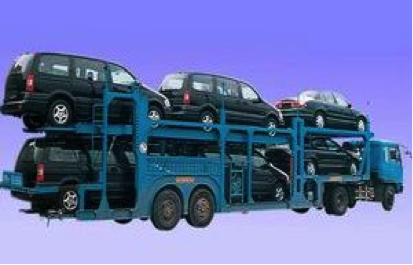
\includegraphics[width=\linewidth]{figure/1-1.png}
  \caption{1-1型轿运车}
\end{minipage}
~
\begin{minipage}[t]{0.32\textwidth}
  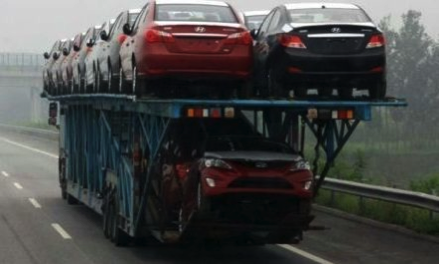
\includegraphics[width=\linewidth]{figure/1-2.png}
  \caption{1-2型轿运车}
\end{minipage}
~
\begin{minipage}[t]{0.32\textwidth}
  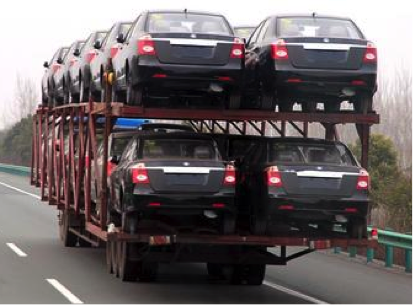
\includegraphics[width=\linewidth]{figure/2-2.png}
  \caption{2-2型轿运车}
\end{minipage}
\end{figure}
%~
%\begin{subfigure}[t]{0.32\textwidth}
%  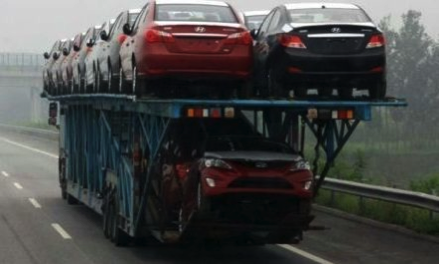
\includegraphics[width=\linewidth]{figure/1-2.png} 
%    \caption{data distribution of \textit{create index}}
%\end{subfigure}
%~
%\begin{subfigure}[t]{0.32\textwidth}
%  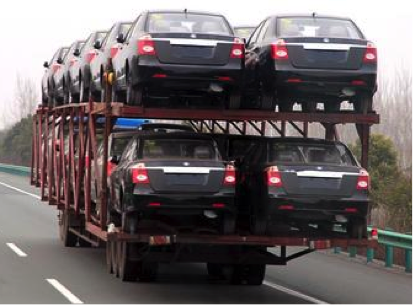
\includegraphics[width=\linewidth]{figure/2-2.png} 
%    \caption{data distribution of \textit{insert table}}
%\end{subfigure}


\subsection{问题要求}
建立数学模型,以通用算法和程序解决整车物流成本优化的问题,能够比较准确得模拟整车物流的装载方案及行车路线,更好地降低整车物流运输成本。
问题一:物流公司要运输Ⅰ车型的乘用车100辆及Ⅱ车型的乘用车68辆。
问题二:物流公司要运输Ⅱ车型的乘用车72辆及Ⅲ车型的乘用车52辆。
问题三:物流公司要运输Ⅰ车型的乘用车156辆、Ⅱ车型的乘用车102辆及Ⅲ车型的乘用车39辆。
问题四:物流公司要运输166辆Ⅰ车型的乘用车(其中目的地是A、B、C、D的分别为42、50、33、41辆)和78辆Ⅱ车型的乘用车(其中目的地是A、C的,分别为31、47辆),具体路线见图4,各段长度:OD=160,DC=76,DA=200,DB=120,BE=104,AE=60。
问题五:附件的表1给出了物流公司需要运输的乘用车类型(含序号)、尺寸大小、数量和目的地,附件的表2给出可以调用的轿运车类型(含序号)、数量和装载区域大小(表里数据是下层装载区域的长和宽, 1-1型及2-2型轿运车上、下层装载区域相同;1-2型轿运车上、下层装载区域长度相同,但上层比下层宽0.8米。此外2-2型轿运车因为层高较低,上、下层均不能装载高度超过1.7米的乘用车。

\section{模型假设}
\begin{enumerate}
	\item 	题目中所列数据均真实可靠;
	\item	乘用车与轿运车两侧的安全距离在说明装载区域大小时已经考虑;
	\item	乘用车不可在轿运车上倾斜摆放;
	\item	轿运车运输路线为有向图;
	\item	运输花费主要由轿运车数量决定,次要由轿运车类型决定。

\end{enumerate}

%\section{基本符号说明}
%	\begin{itemize}
%		\item $i$乘用车索引,
%	\end{itemize}


\section{问题分析}
\subsection{问题一、二、三分析}
问题一、二、三要求计算各种类型轿运车的数量和每辆轿运车的乘用车装载方案,各类型乘用车数量已知,所需各类型轿运车数量及各轿运车的装载方案未知。
针对题中给出的轿运车、乘用车信息,可以抽象为一个三维装箱问题,从长、宽、高三个维度来建立模型。并采用约束编程的思想,将题中提到的约束条件:安全距离、乘用车规格、轿运车使用量等约束条件翻译成机器能够识别的信息,以缩小模型的解空间。之后设定目标函数,即表示总成本的函数,使用Gecode运算框架快速解出最小总成本的乘用车装载方案。


\subsection{问题四分析}

\section{模型的建立与求解}

\subsection{问题一、二、三通用}

\subsubsection{模型建立}
	\paragraph{实例变量}
	\paragraph{决策变量}
	\paragraph{约束条件}

\subsubsection{模型求解}
本模型是基于约束编程的思想所建立,模型的求解使用Gecode \cite{gecode}

\section{模型的评价、改进及推广}



\begin{thebibliography}{1}  % even better: use BibTeX!
\bibitem{gecode} Gecode Team.  \textit{Gecode}: Generic Constraint
  Development Environment, 2006.  

%\bibitem{Search} Simonis, Helmut, and Barry O’Sullivan. "Search strategies for rectangle packing." \emph{Principles and Practice of Constraint Programming.} Springer Berlin Heidelberg, 2008.

\end{thebibliography}

\appendix
\section{代码}




\end{document}